\documentclass[10pt,twocolumn]{article}
\usepackage[a4paper,margin=0.55in,columnsep=0.22in]{geometry}
\usepackage{graphicx,booktabs,amsmath,siunitx,xcolor}
\usepackage[font=footnotesize,labelfont=bf,skip=2pt]{caption}
\usepackage[hidelinks]{hyperref}
\usepackage{titlesec}
\titlespacing*{\section}{0pt}{5pt}{2pt}
\titlespacing*{\subsection}{0pt}{3pt}{1pt}
\titleformat*{\section}{\normalsize\bfseries}
\titleformat*{\subsection}{\small\bfseries}
\setlength{\parskip}{1pt}
\setlength{\textfloatsep}{5pt}
\setlength{\floatsep}{4pt}
\setlength{\dbltextfloatsep}{5pt}
\sisetup{group-minimum-digits=4}
\newcommand{\tps}{tok/s}

\title{\vspace{-0.6in}\large\textbf{Dense vs.\ small mixture-of-experts LLMs on a CPU, and a Mamba-3 decode step}\\[1pt]
\normalsize CPU Inference Project --- Option 6 (small MoE) with Option 1 (dense) as baseline, plus the Mamba-3 bonus}
\author{\vspace{-0.35in}}
\date{}

\begin{document}
\maketitle
\vspace{-0.25in}

\section{Question, hardware and setup}
\textbf{Questions.} For the Granite-3.1 MoE models (1B-A400M, 3B-A800M) against the dense Llama-3.2 models of the same
total size (1B, 3B): does decode speed follow \emph{active} or \emph{total} parameters, what does expert routing cost, how
close does decode get to the memory-bandwidth limit, and when does attention start to dominate as context grows?

\textbf{Hardware.} At the team's request we used a cluster node instead of a laptop: Intel Xeon Platinum 8480+
(Sapphire Rapids), 2 sockets $\times$ 56 cores (homogeneous, no P/E split), 48\,KiB L1d / 2\,MiB L2 per core, 105\,MiB
L3 per socket, AVX2 + AVX-512 (F/BW/VL/VNNI/BF16; AMX is present but not exposed by kernel 5.4), 503\,GB DDR5.
To stay comparable with the brief, \emph{every} run uses one socket: physical cores only, memory bound to that NUMA node,
threads pinned (\texttt{numactl}, \texttt{OMP\_PLACES=cores}). Core~1 is excluded because the storage daemon keeps it busy
(\S\ref{sec:threads} shows why that matters), so ``all performance cores'' is 55. Bandwidth on that socket
(STREAM + a read-only SIMD reduction) is in Table~\ref{tab:bw}. Decode is read-dominated, so the roofline uses the
read-only number: \textbf{13.6\,GB/s on one core, saturating at $\approx$136\,GB/s from 16 cores} (2--3$\times$ a laptop,
so absolute \tps\ are higher than on a laptop, but the reasoning is the same).

\textbf{Software.} llama.cpp \texttt{e30ad80}, CPU-only (\texttt{-march=native}, OpenMP, gcc 9.4); F16 GGUFs quantized
locally to Q4\_K\_M (all models) and Q8\_0 (models $\le$1.5B). Weights are loaded without mmap so peak RSS (recorded for every
run with \texttt{/usr/bin/time}) is not double counted; no run exceeded 4.5\,GB (max 4.05\,GB, Llama-3B at 8k; Fig.~\ref{fig:mem}) and none
swapped. Every point is the mean of 3 separate processes; error bars are $\pm$1 s.d. The node is shared, so the load
average is logged with each run. Decode at context $C$ is \texttt{llama-bench -n 128 -d $C$-128}; context caps are 16k (1B
class) and 8k (3B class). Everything is scripted (\texttt{scripts/run\_all.sh}); raw CSVs are in \texttt{results/csv}.

\begin{table}[t]\centering\footnotesize\setlength{\tabcolsep}{3.5pt}
\caption{Memory bandwidth on one socket (GB/s, mean of 3).}\label{tab:bw}
\begin{tabular}{lrrrrrrr}\toprule
threads & 1 & 2 & 4 & 8 & 16 & 32 & 55\\\midrule
read-only & 13.6 & 27.0 & 50.7 & 92.7 & 133.7 & 135.7 & 133.9\\
STREAM Copy & 21.6 & 41.3 & 69.9 & 101.5 & 116.1 & 117.1 & 114.6\\
STREAM Triad & 14.4 & 28.1 & 49.8 & 78.4 & 94.7 & 108.5 & 121.6\\\bottomrule
\end{tabular}\end{table}

\textbf{Correctness.} WikiText-2 test (first 100k characters, ctx 512): Q8\_0 is within 0.1--0.4\% of F16 perplexity,
Q4\_K\_M costs 3.1--3.4\% (Llama) and 5.8--7.2\% (Granite) (Llama-1B 14.59/14.12/14.11, Llama-3B 10.63/--/10.31,
Granite-1B 8.82/8.36/8.33, Granite-3B 7.72/--/7.20 for Q4/Q8/F16; F16 is a reference only, never benchmarked). Greedy chat
outputs are coherent for all six models (\texttt{results/raw/samples}).

\section{Predict before measuring}
Bytes per decoded token at batch 1 are read off the GGUF tensor table: all non-expert weights, only the
$k/E$ routed fraction of the expert tensors, the LM head (both families \emph{tie} embeddings, so the Q6\_K embedding
matrix is read in full every token: 215\,MB, 27\% of Llama-1B) and the whole KV cache (F16).
\begin{table}[t]\centering\scriptsize\setlength{\tabcolsep}{2.2pt}
\caption{Roofline inputs (parameters; GB read per token; KV cache KiB per context token) and prediction (read BW at 32 threads) vs.\ measured decode (\tps, 32 threads, tg128).}\label{tab:bytes}
\begin{tabular}{lrrrrrr}\toprule
model & total & active & GB/tok & KV & pred. & meas.\\\midrule
Llama-1B Q4  & 1.24B & 1.24B & 0.80 & 32 & 169 & 134\\
Llama-1B Q8  & 1.24B & 1.24B & 1.31 & 32 & 103 & 87\\
Llama-3B Q4  & 3.21B & 3.21B & 2.01 & 112 & 67 & 54\\
Granite-1B Q4 & 1.33B & 0.43B & 0.27 (0.82) & 48 & 494 (165) & 222\\
Granite-1B Q8 & 1.33B & 0.43B & 0.46 (1.42) & 48 & 294 (95) & 169\\
Granite-3B Q4 & 3.30B & 0.88B & 0.55 (2.02) & 64 & 244 (67) & 130\\\bottomrule
\end{tabular}\\[1pt]{\scriptsize In parentheses: if all experts were read (total parameters).}
\end{table}

\section{Results}
\label{sec:threads}
\begin{figure*}[t]\centering
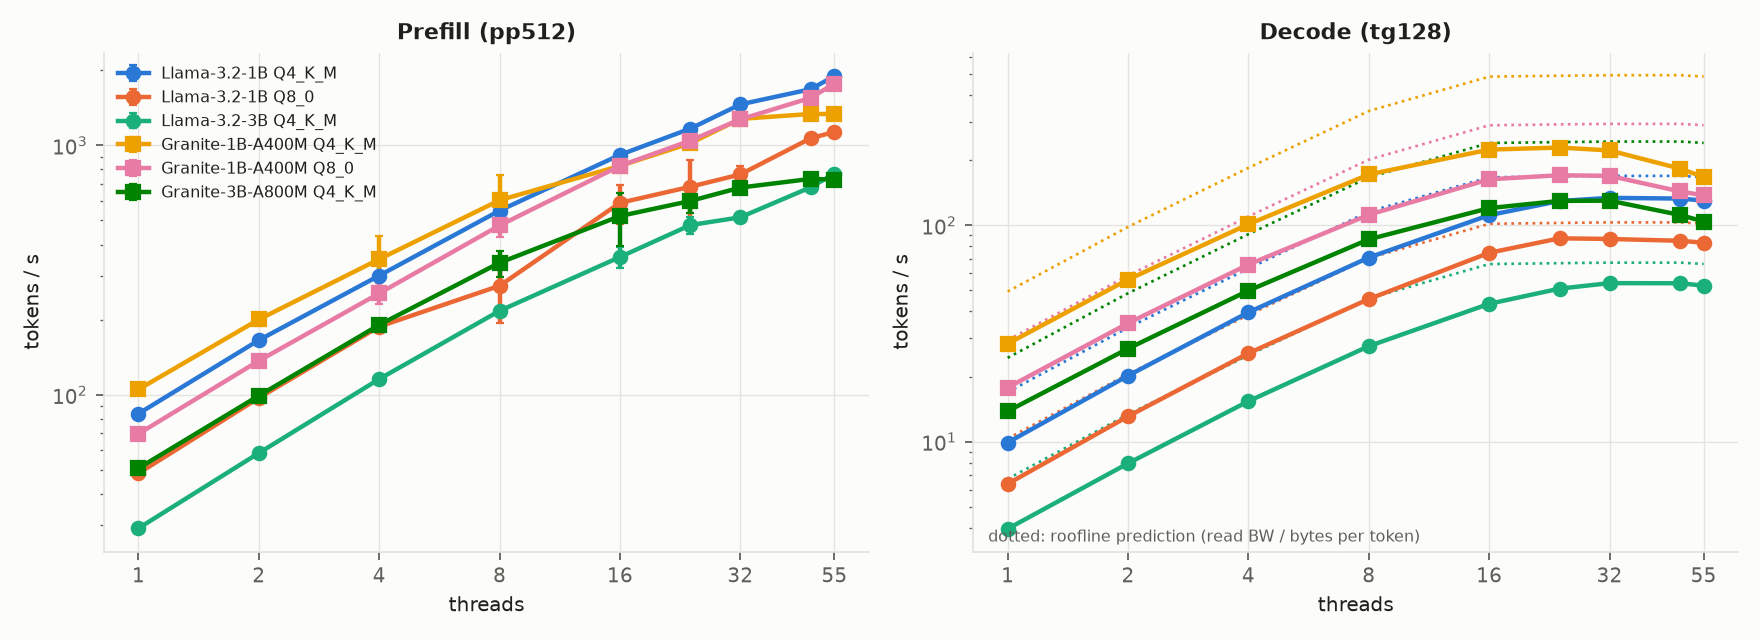
\includegraphics[width=0.66\textwidth]{../plots/thread_scaling.png}%
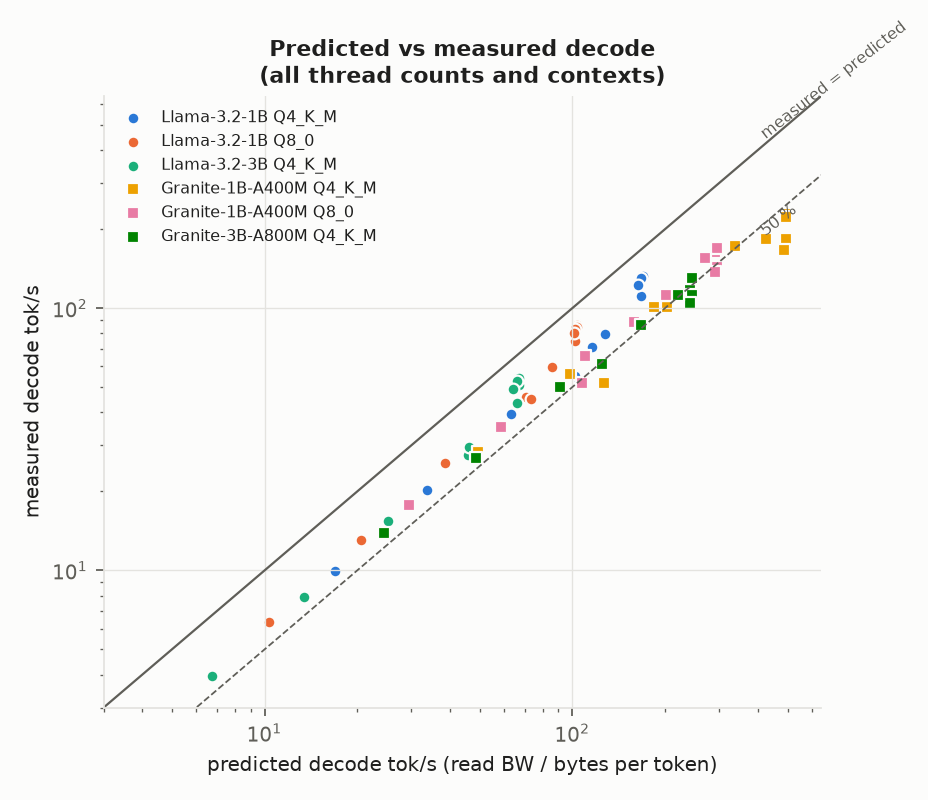
\includegraphics[width=0.33\textwidth]{../plots/pred_vs_measured.png}
\caption{Left: thread scaling of prefill (pp512) and decode (tg128); dotted = roofline prediction. Right: predicted vs.\ measured decode
for every thread count and context.}\label{fig:threads}
\end{figure*}

\textbf{Thread scaling (Fig.~\ref{fig:threads}).} Prefill is compute-bound and keeps scaling to 55 cores (Llama-1B Q4:
84\,$\to$\,1895\,\tps, 22.6$\times$). Decode tracks bandwidth: it scales almost linearly to 8 threads, then flattens where
bandwidth saturates (16--24 threads) and \emph{drops} beyond 32 threads for the MoE models (Granite-1B: 229 at 24 threads,
167 at 55). Pinning matters: with core~1 (busy with a system daemon) inside the pinned set, the shared reference test fell from
${\approx}$1450 to 190\,\tps\ prefill and from ${\approx}$130 to 9\,\tps\ decode, because every graph node waits at a barrier for
the slowest thread.

\textbf{How close to the roofline.} Dense decode reaches only 58--63\% of the prediction on 1--8 threads: there one core cannot
dequantize Q4\_K fast enough to keep its memory stream busy (Q8\_0, cheaper to unpack, reaches 62--67\%). From 24 threads,
where the socket's bandwidth is the limit, dense models reach 77--85\%. MoE models stay at 45--58\% and fall to 34--47\% at 55
threads.

\begin{figure*}[t]\centering
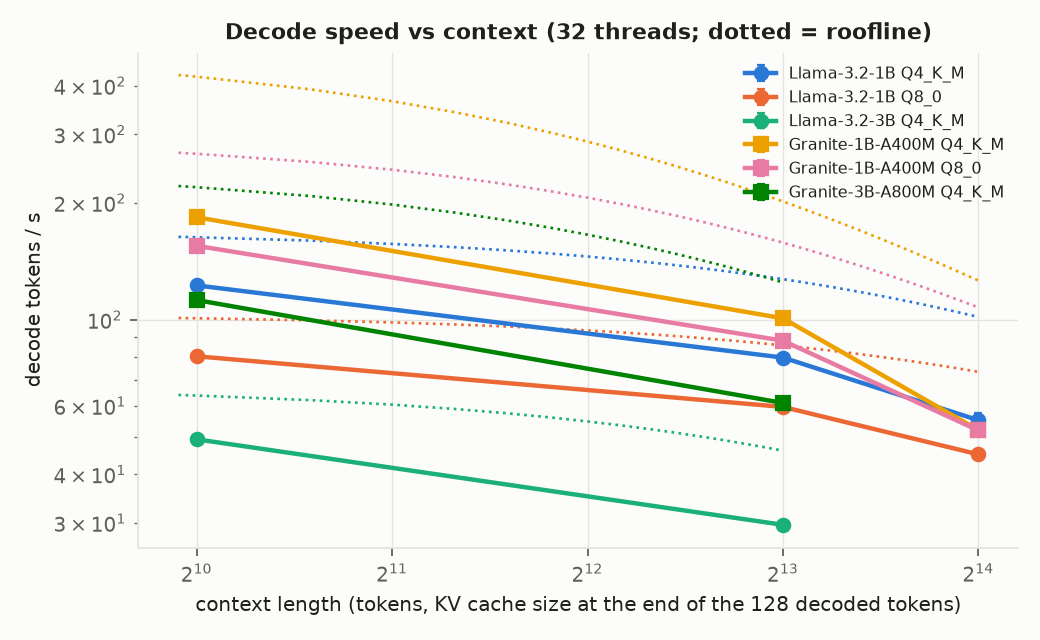
\includegraphics[width=0.36\textwidth]{../plots/decode_vs_context.png}%
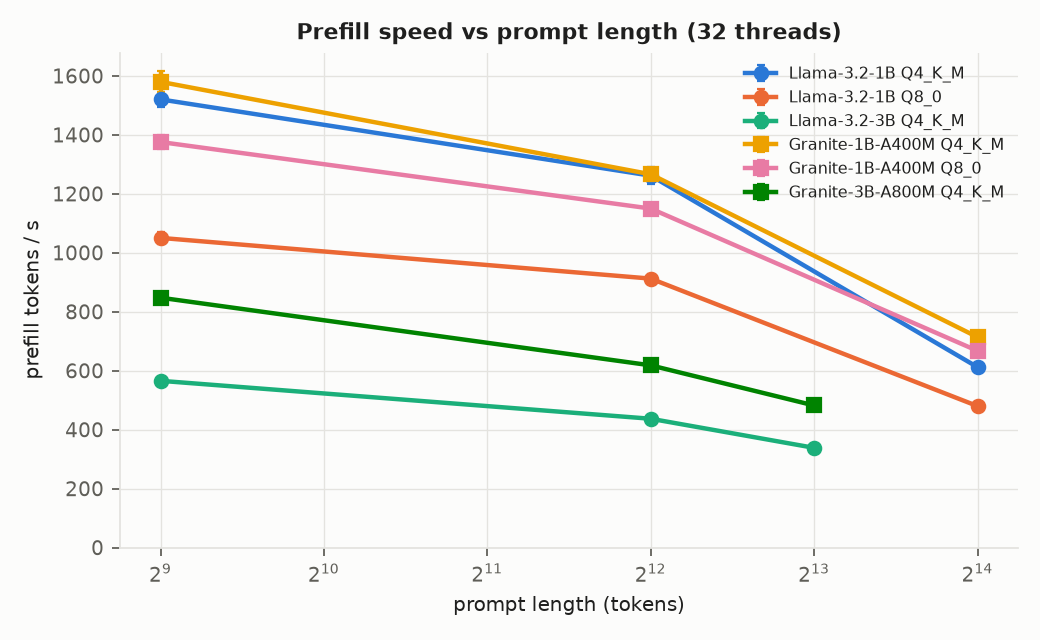
\includegraphics[width=0.32\textwidth]{../plots/prefill_vs_prompt.png}%
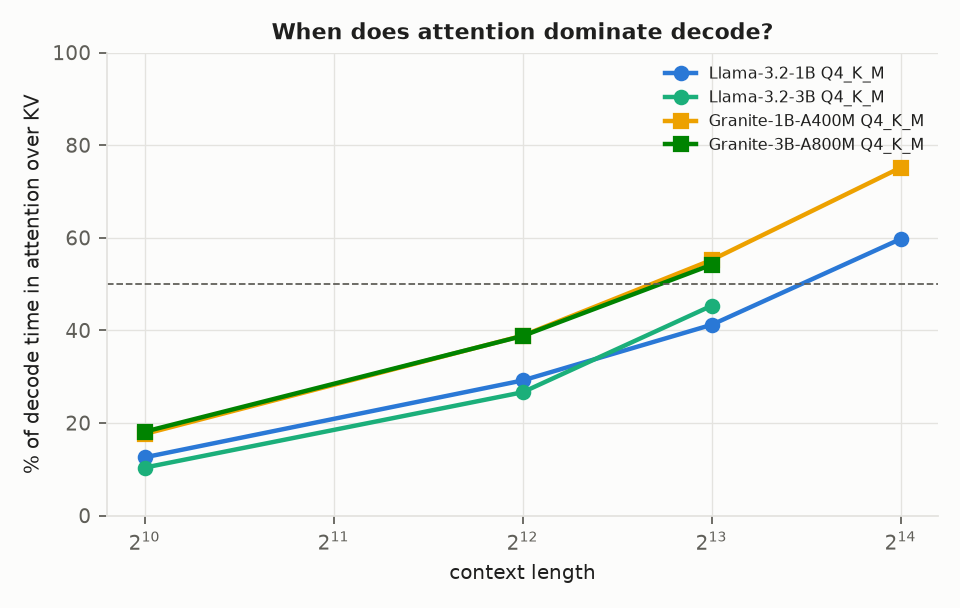
\includegraphics[width=0.32\textwidth]{../plots/attention_share.png}
\caption{Left: decode vs.\ context (dotted: roofline incl.\ KV). Middle: prefill vs.\ prompt length. Right: share of decode time in
attention over the KV cache (from the profile).}\label{fig:context}
\end{figure*}

\textbf{Context length (Fig.~\ref{fig:context}).} Prefill falls with prompt length (Llama-1B: 1520 at 512, 612 at 16k) as the
quadratic attention work grows. Decode slows faster than the bytes predict: from 1k to 16k Llama-1B goes 122\,$\to$\,55\,\tps\
(roofline: 163\,$\to$\,102), and Granite-1B 183\,$\to$\,52, ending \emph{slower} than the dense model because its KV cache is
larger (48 vs.\ 32\,KiB/token) while its weight savings no longer matter. Attention over the KV cache passes 50\% of decode time
between 4k and 8k for the MoE models and between 8k and 16k for the dense ones.

\section{Profiling}
\texttt{perf} is blocked on this cluster (\texttt{perf\_event\_paranoid}\,=\,3), so we added an opt-in per-operator timer to the
ggml CPU graph loop (\texttt{patches/ggml\_op\_profile.patch}, compiled only into a separate build). Thread~0 timestamps each node
at its start, when its own share ends, and after the barrier that closes it, so we get op time, own compute, and barrier wait.
Node names are kept, so the routing ops are visible individually.

\begin{figure*}[t]\centering
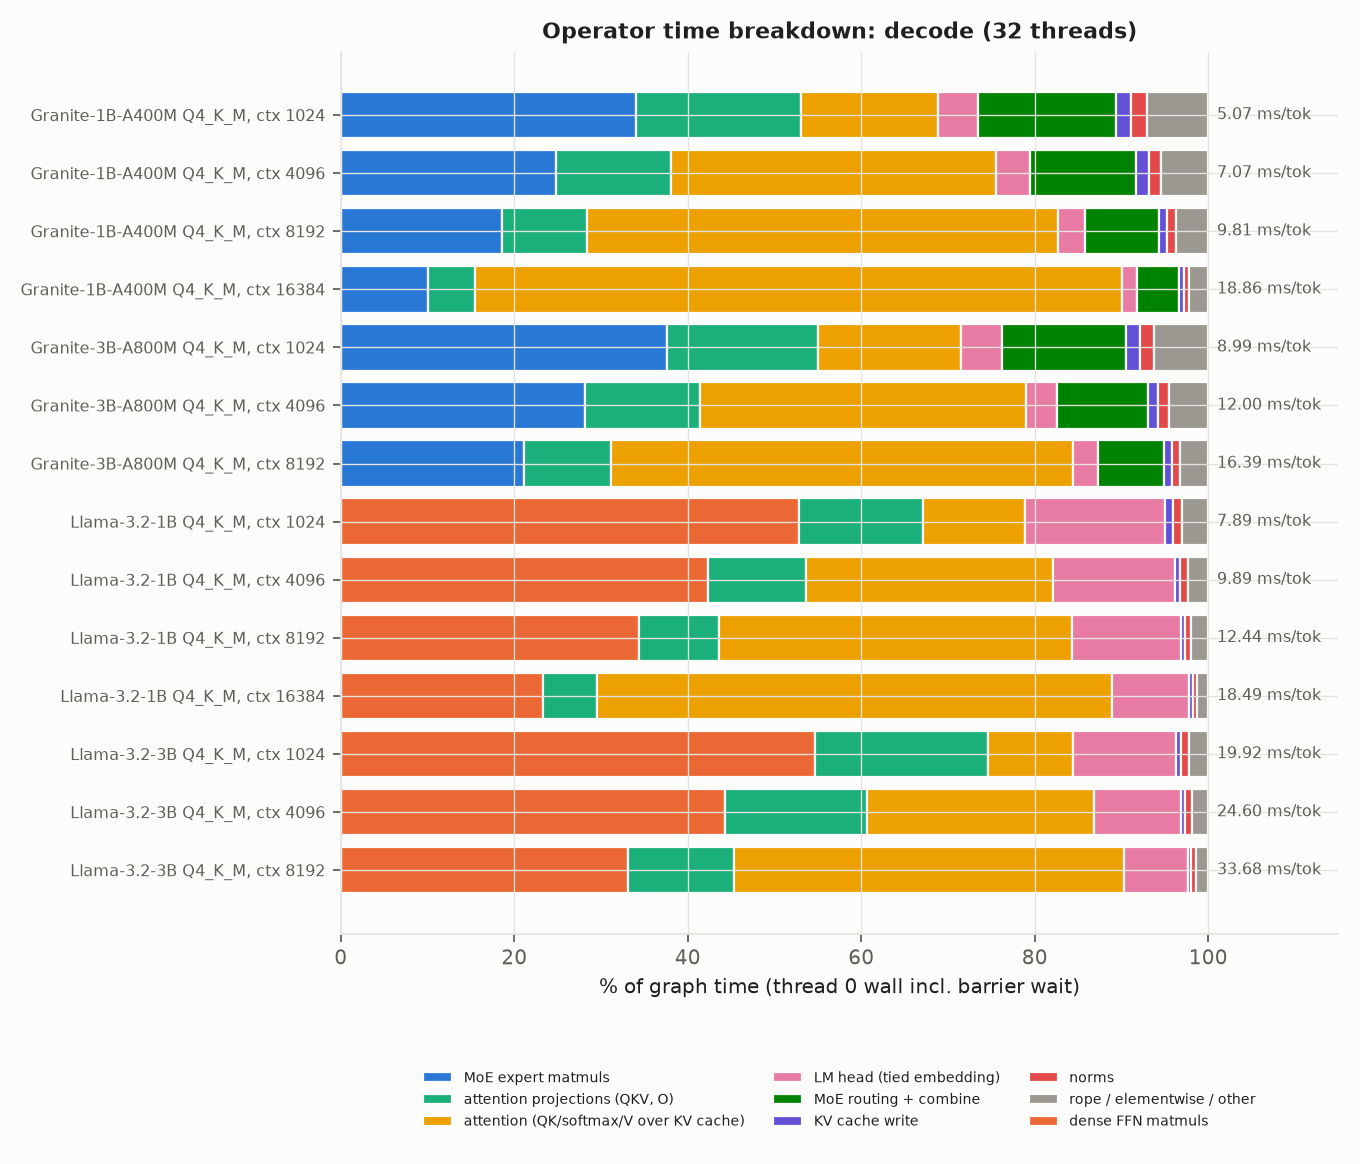
\includegraphics[width=0.62\textwidth]{../plots/op_breakdown_decode.png}%
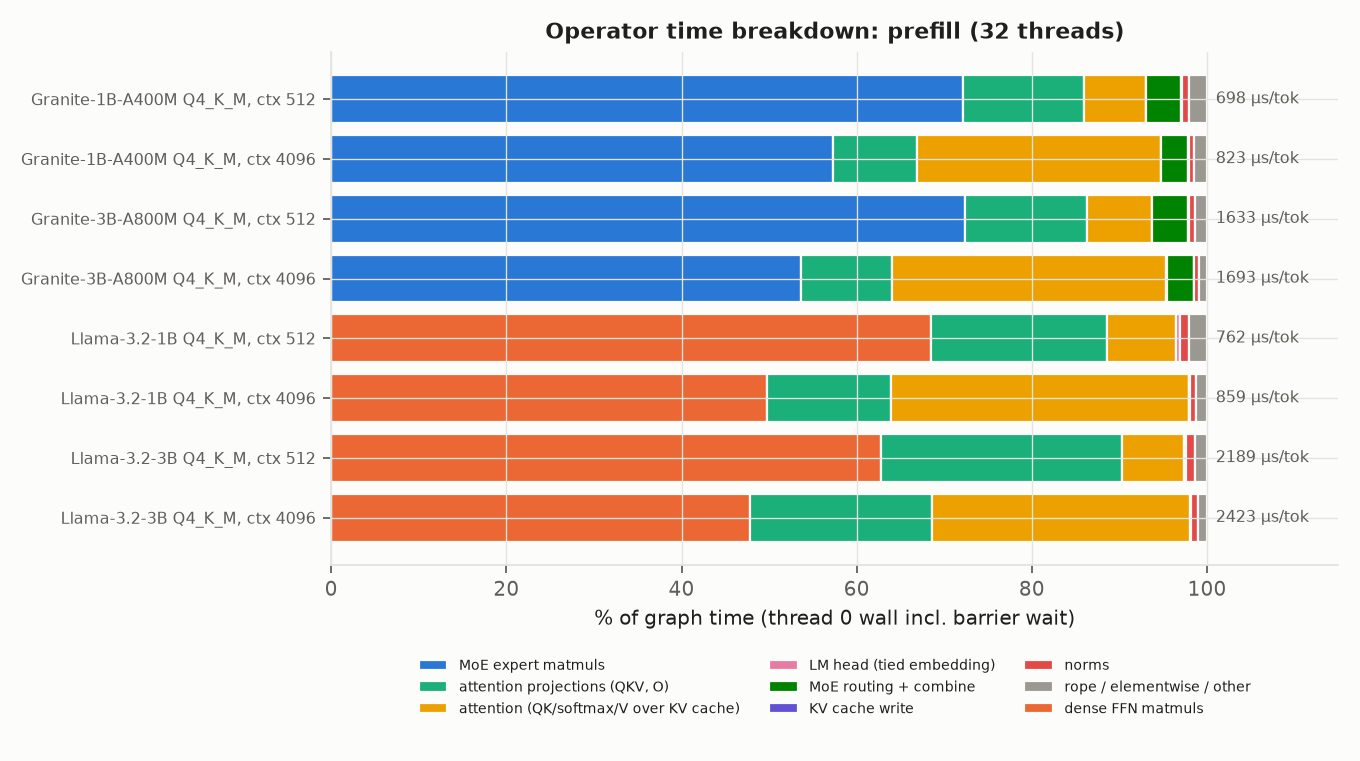
\includegraphics[width=0.38\textwidth]{../plots/op_breakdown_prefill.png}
\caption{Time by operator group at 32 threads: decode (left, per context) and prefill (right). Bar length is wall time including
barrier wait; totals in ms (decode) or \textmu s (prefill) per token.}\label{fig:ops}
\end{figure*}

\textbf{Top operators.} Prefill: the three FFN matmuls (dense) or the three \texttt{MUL\_MAT\_ID} expert matmuls (MoE),
69--74\% together. Decode at 1k: dense: \texttt{ffn\_down}, LM head, \texttt{ffn\_gate} (21/16/16\%, Llama-1B); MoE:
\texttt{FLASH\_ATTN\_EXT}, \texttt{ffn\_moe\_down}, \texttt{ffn\_moe\_gate} (15/12/10\%, Granite-1B). Fig.~\ref{fig:ops} shows
the groups.

\textbf{What routing costs.} The router GEMV, softmax, argsort/top-k, gather, normalise and weight ops plus the add-up of the
8 expert outputs take 0.80\,ms/token, 15\% of Granite-1B decode at 1k (14\% for 3B, 5\% at 16k). Almost none of it is
arithmetic: e.g.\ the weight normalisation spends 2.6\,\textmu s of its 45\,\textmu s per token computing; the rest is waiting at
its barrier. The MoE graph has 823 nodes per token against 277 for Llama-1B, and at 32 threads barrier wait totals
1.23\,ms/token (25\% of Granite-1B decode vs.\ 10\% for Llama-1B). On one thread, where there is no barrier, the same graph
costs 48\,ms/token vs.\ 116 for Llama-1B (2.4$\times$ faster), which is close to the 2.9$\times$ byte ratio.

\begin{figure*}[t]\centering
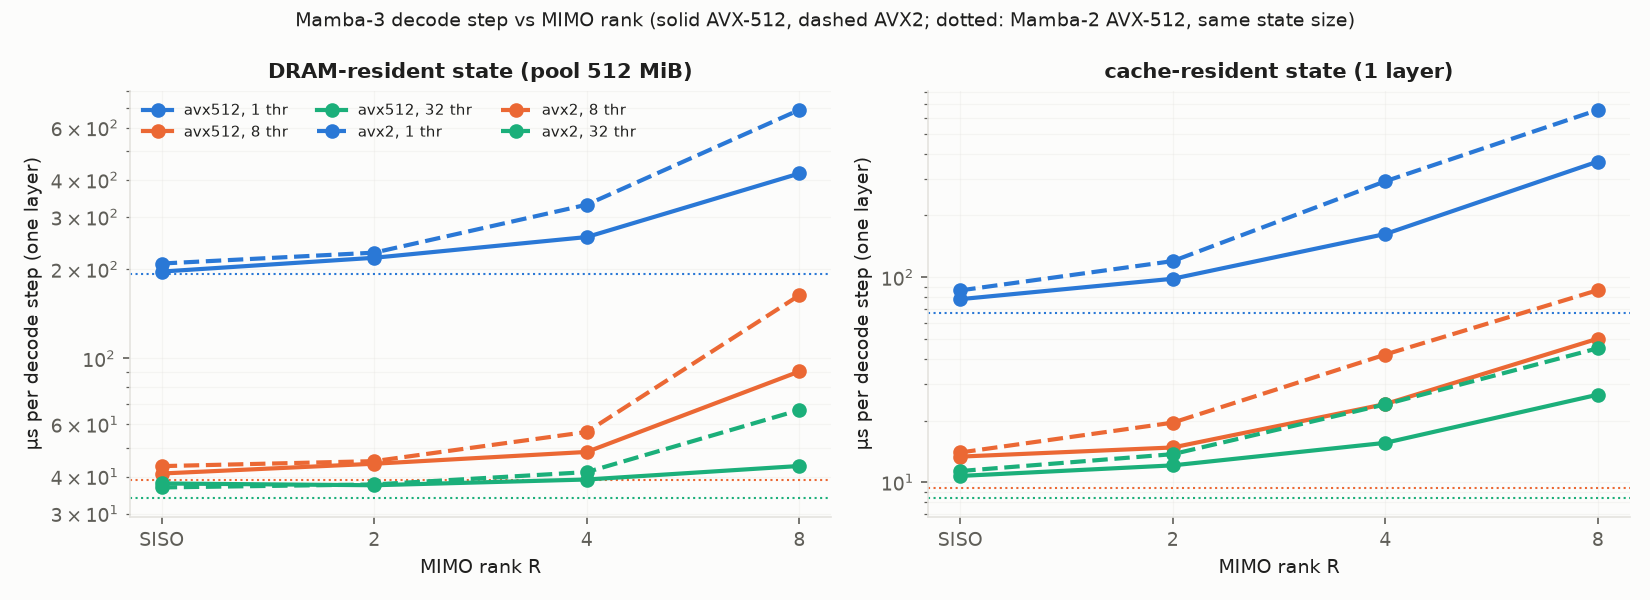
\includegraphics[width=0.66\textwidth]{../plots/m3_time_vs_rank.png}%
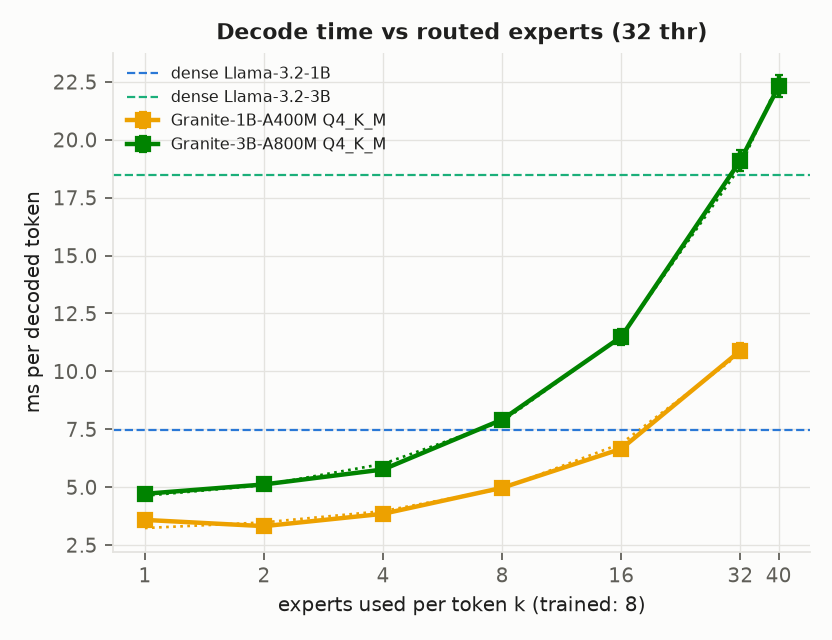
\includegraphics[width=0.33\textwidth]{../plots/experts_k_left.png}
\caption{Left: one Mamba-3 layer decode step (64 heads $\times$ 64 $\times$ 128 state, 2\,MiB) vs.\ MIMO rank, state in DRAM and in
cache; dotted: Mamba-2 at the same state size. Right: own experiment, decode time vs.\ experts per token.}\label{fig:m3}
\end{figure*}
\section{Explaining the gap to the roofline}
(1)~\emph{Compute-bound dequantization on few cores}: Q4\_K unpacking keeps single-core decode at ${\approx}$60\% of the
read bandwidth. (2)~\emph{Synchronisation}: one barrier per graph node costs 1.5--3\,\textmu s at 32 threads; it is 8--10\% of
dense decode but 23--25\% of MoE decode, and grows with thread count, which is why MoE decode peaks at 24--32 threads.
(3)~\emph{Attention inefficiency at long context}: single-query flash attention reads the KV cache at well below stream bandwidth
(Llama-1B at 16k: 59\% of time in attention for 40\% of the bytes). (4)~\emph{Small MoE matmuls}: an 8-of-32 expert GEMV over
512-wide experts has too little work per thread to reach full bandwidth. Thermal throttling was not observed (server cooling; 3 reps
agree within 1--2\% at high thread counts).

\begin{figure}[t]\centering
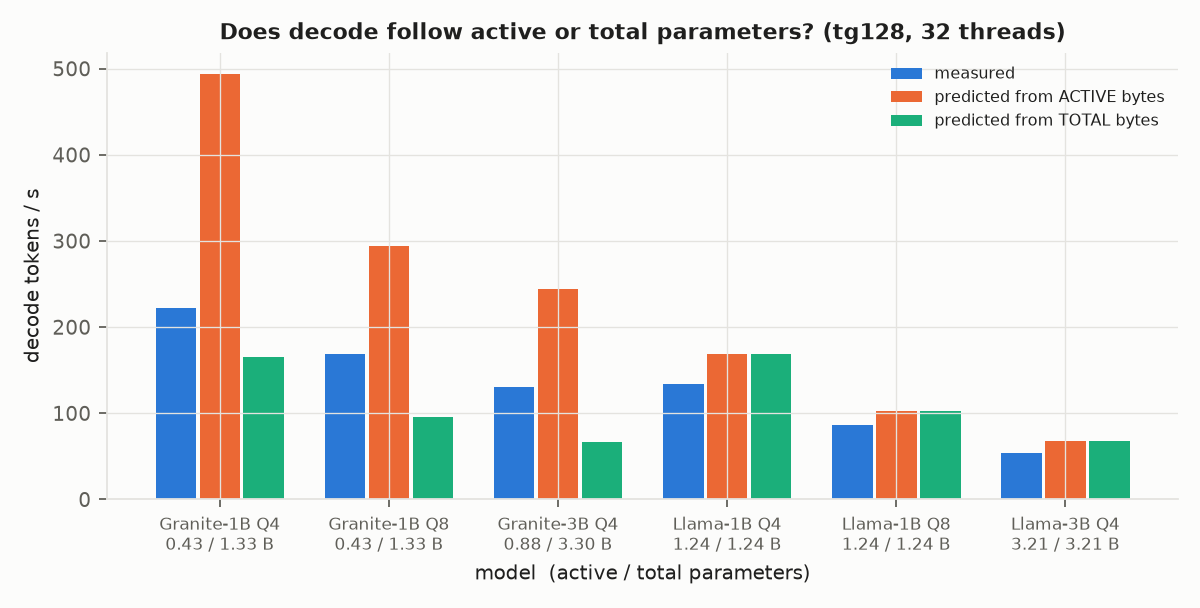
\includegraphics[width=\columnwidth]{../plots/active_vs_total.png}
\caption{Measured decode vs.\ the roofline from active and from total bytes (32 threads).}\label{fig:active}
\end{figure}
\textbf{Active or total?} Decode follows \emph{active} parameters, but only partly: at 32 threads Granite-1B decodes 1.66$\times$
faster than Llama-1B (bytes predict 2.9$\times$) and Granite-3B 2.4$\times$ faster than Llama-3B (bytes: 3.6$\times$). All MoE
points sit far above the ``total bytes'' prediction (Table~\ref{tab:bytes}, Fig.~\ref{fig:active}). Prefill does not benefit from sparsity: with 512
tokens every expert is used, and Granite-1B prefill (1580\,\tps) equals Llama-1B (1520).

\section{Our experiment: number of routed experts $k$}
We rewrote \texttt{expert\_used\_count} in copies of the GGUF (\texttt{scripts/experiment\_experts.py}), so the file and the
\emph{total} parameters are unchanged while the \emph{active} ones vary, and measured decode, prefill and perplexity for
$k\in\{1,\dots,32\}$ ($k$=40 = all experts for 3B). llama.cpp sizes its graph for the trained $k$=8, so $k>8$ overflowed the node table; a
6-line, \texttt{\#ifdef}-guarded patch adds headroom in a separate build used for every $k$ (its $k$=8 numbers are within 3--5\% of the main
build). \textbf{Decode time is linear in $k$} (Fig.~\ref{fig:m3}, right): 243\,\textmu s per extra expert for Granite-1B and 458\,\textmu s
for 3B, against 168 and 336\,\textmu s from the bytes per expert at 136\,GB/s, so expert weights stream at ${\approx}$70\% of bandwidth.
This is the direct answer to ``active or total'': with total parameters fixed, time follows the active ones. Two further results: below
$k$=4 time stops falling (3.3--3.6\,ms floor of attention, projections, LM head and synchronisation), and with all experts active
(0.82\,GB/token) Granite-1B takes 10.9\,ms/token vs.\ 7.5 for Llama-1B (0.80\,GB): the MoE machinery itself costs 1.45$\times$ at equal
bytes (1.2$\times$ for 3B). Quality is best at the trained $k$: perplexity 8.8 at $k$=8, 22 at $k$=4, 11 at $k$=16, $>$3000 at $k\le2$.
Prefill speed scales like $1/k$ (Granite-1B 2632 to 397\,\tps\ for $k$=1 to 32) because every token runs $k$ expert matmuls.

\begin{figure}[t]\centering
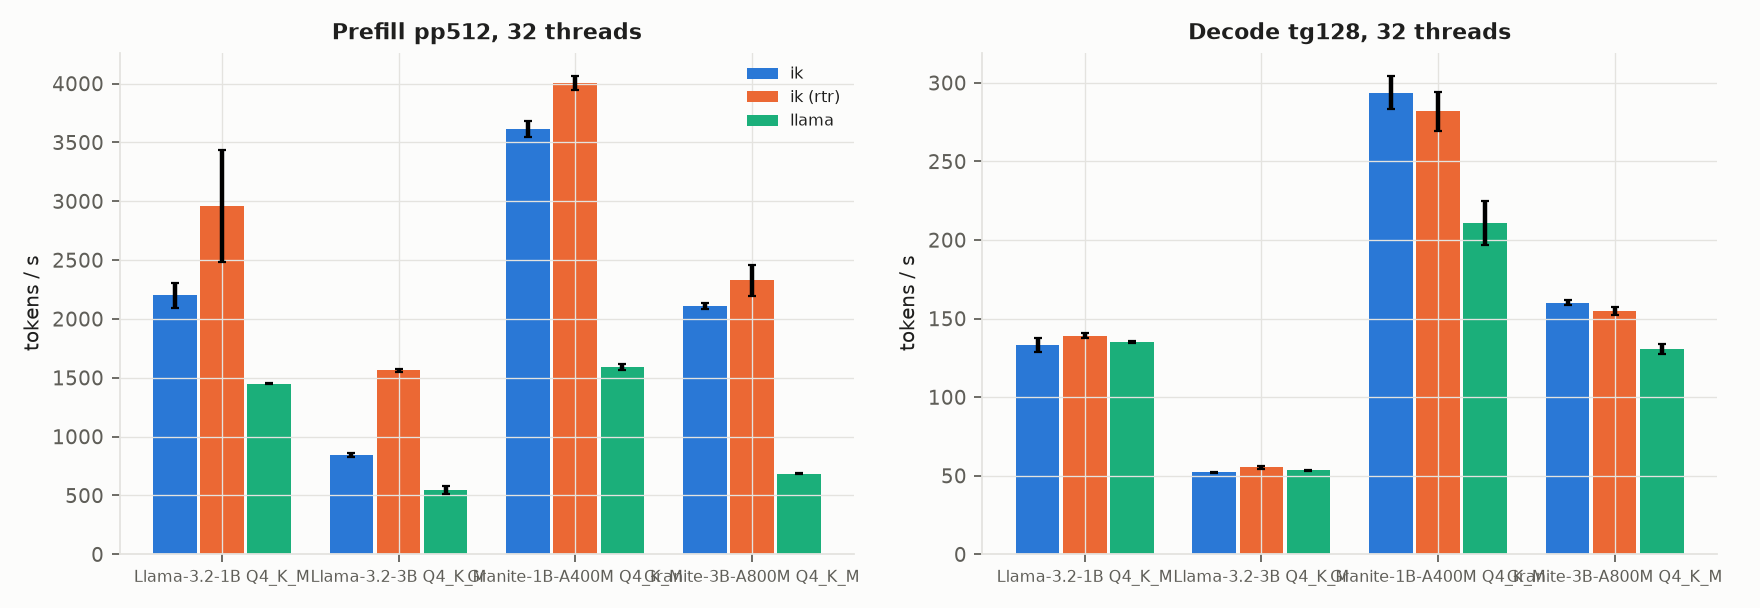
\includegraphics[width=\columnwidth]{../plots/ik_vs_llamacpp.png}
\caption{llama.cpp vs.\ ik\_llama.cpp (default, and with run-time repacking), same GGUFs and pinning, 32 threads.}\label{fig:ik}
\end{figure}
\begin{figure}[t]\centering
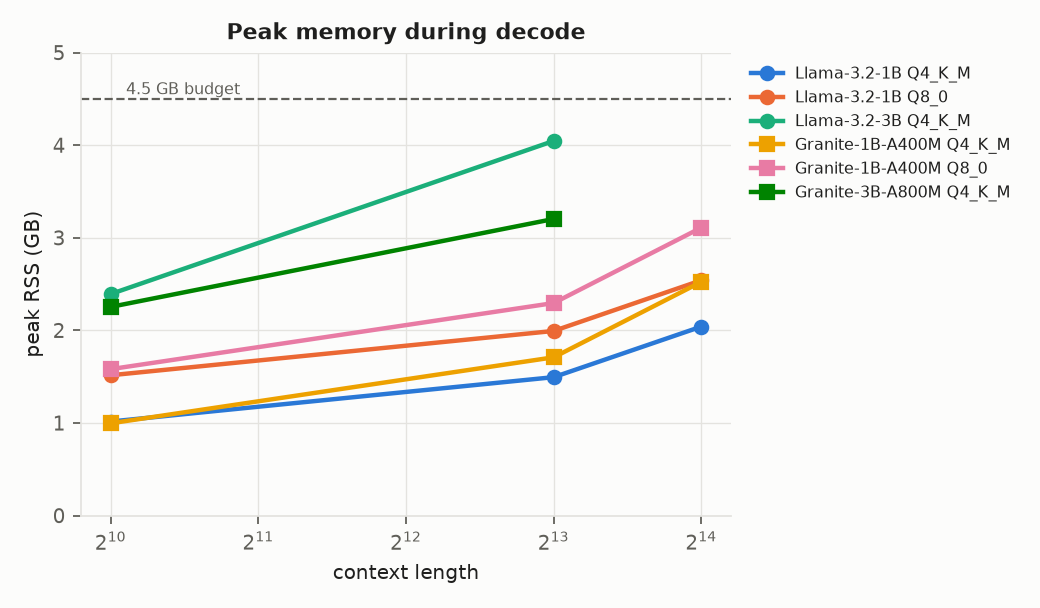
\includegraphics[width=0.85\columnwidth]{../plots/memory_vs_context.png}
\caption{Peak RSS during decode vs.\ context; every run stays under the 4.5\,GB budget.}\label{fig:mem}
\end{figure}
\textbf{Stretch: ik\_llama.cpp} (Fig.~\ref{fig:ik}). Same GGUFs, same pinning (built with GCC 9 plus two small compatibility shims). Its fused MoE
kernel removes most of the routing nodes: Granite-1B decode 294 vs.\ 211\,\tps\ (+39\%), Granite-3B 160 vs.\ 131 (+22\%),
prefill 2.3$\times$ and 3.1$\times$ faster (2.5$\times$/3.4$\times$ with run-time repacking). Dense decode is unchanged (within 3\%),
which supports the synchronisation explanation above. \textbf{Shared reference test} (Llama-1B Q4\_K\_M, pp512 + tg128):
1873\,\tps\ prefill and 124\,\tps\ decode on 55 cores (1784 / 129 on 32 cores; s.d.\ $<$3\%) on this node; the PARAM Rudra job script is \texttt{scripts/rudra\_reference.sbatch}.

\section{Bonus: a Mamba-3 decode step on CPU}
We implemented the SISO and MIMO step (exponential-trapezoidal update, data-dependent RoPE on B/C, MIMO x/z/out projections) in
C++ from one source compiled to scalar, AVX2, AVX-512 and NEON. The official PyTorch reference functions are extracted verbatim from
\texttt{state-spaces/mamba} and run on CPU in fp64. Over 1000 steps every kernel (3 ISAs $\times$ 1/8 threads $\times$ SISO, MIMO
$R$=1/2/4/8, Mamba-2, and layer~0 of the released \texttt{mamba3-siso-1.5b} and \texttt{mamba3-mimo-1.5b} on real token embeddings)
matches within the stated tolerance $10^{-5}$ (output error $1$--$3.5\times10^{-7}$, at or below PyTorch's own fp32 run). Keeping the
RoPE angle accumulator in fp64 was necessary: in fp32 it drifted $4\times10^{-5}$\,rad on the real SISO layer. Vectorising
\texttt{exp}/\texttt{sincos} (the SiLU gates and RoPE were the hidden bottleneck) and register-blocking state rows made MIMO-4 1.6$\times$
faster. The kernel also runs as a ggml custom op in a ggml graph, bit-identical to the direct call; our Mamba-2 step is 3$\times$ faster
than ggml's \texttt{SSM\_SCAN} on one core (88 vs.\ 272\,\textmu s; ggml writes the state out of place).

\textbf{Does MIMO's extra compute come at little cost?} MIMO-4 does 3.6$\times$ the FLOPs of SISO on the same state (arithmetic
intensity 0.85\,$\to$\,2.9\,FLOP/B). With the state in DRAM, as in a deep model, it costs 1.31$\times$ on one AVX-512 core (196 vs.\
257\,\textmu s), 1.18$\times$ on 8 cores and 1.03$\times$ at 32 cores, where the step streams state at the socket's 114\,GB/s, so there
it is effectively free, as on a GPU. With AVX2 only, as on most laptops, it is 1.58$\times$ on one core, and with the state in cache it
becomes compute-bound (1.8$\times$ on 8 cores). Per full layer, the Q4\_K\_M in/out projections (14.7 vs.\ 15.6\,MB) dominate, so
MIMO-4 adds $\approx$10\% per decode step (1279 vs.\ 1405\,\textmu s on 1 core; 200 vs.\ 216 on 8). Our answer: not free inside the
kernel on a laptop-class core, cheap at the level of a decode step, and free once decode is bandwidth-bound.

\section{What we learned}
On a CPU, decode is a memory-streaming problem only when enough cores run: on few cores dequantization is the limit, and on many
cores the barrier after every graph node is. Sparsity (MoE) cuts bytes 3$\times$ but adds 3$\times$ the graph nodes, so on CPU it
pays about half of what the bandwidth model promises, and less at long context, where the KV cache dominates. Fusing the MoE ops
(ik\_llama.cpp) recovers much of the gap. Measure on pinned, quiet cores: one busy core cost us 10$\times$.

\end{document}
